\documentclass{article}
\usepackage[T1]{fontenc}
\usepackage{lmodern}
\usepackage{graphicx}
\usepackage{amsmath,amssymb}
\usepackage[a4paper,margin=2cm]{geometry}
\usepackage[absolute,overlay]{textpos}
\setlength{\TPHorizModule}{1mm}
\setlength{\TPVertModule}{1mm}
\usepackage[indonesian]{babel}
\usepackage{hyperref}
\setlength{\emergencystretch}{2em}
% unit: Halaman 97

\begin{document}

% === Halaman 97 (python/native) ===

97

• Contoh:



K = 

 Plainteks: paymoremoney

 Enkripsi tiga huruf pertama: pay = (15, 0, 24)


   Cipherteks: C = 



                           = LNS


 Cipherteks selengkapnya: LNSHDLEWMTRW





















19

2

2

21

18

21

5

17

17





















=





















=









































18

13

11

26

mod

486

819

375

24

0

15

19

2

2

21

18

21

5

17

17

% deskripsi: gambar native xref 338
\noindent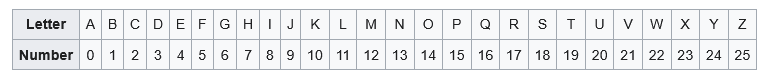
\includegraphics[width=0.85\textwidth]{../../images/python/page_097_img_01.png}

\end{document}
